This section evaluates the sensing redundancy and channel-localization components of the proposed framework using a water-distribution CPS. The available data establish the empirical observability profile and quantify the effect of physics-guided attack data on localization. The scope of the study is limited to these two components; no KF/$\chi^2$ performance claim is inferred from residual-based simulations of the earlier estimator.

\subsection{Water-distribution model}
The system in Fig.~\ref{fig:water_distribution_sys} contains ten operating tanks and one storage tank. The control objective is to regulate the operating-tank levels by adjusting the inlet valves. Random consumer demand is modeled as a process disturbance. Level and differential-pressure measurements are transmitted to the control center and may be compromised by additive FDIAs.

\begin{figure}[!ht]
    \centering
    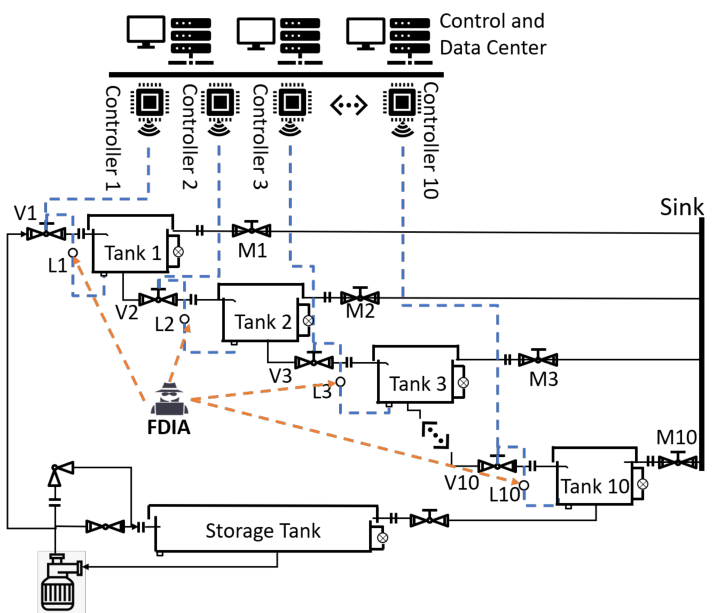
\includegraphics[width=\columnwidth]{image/WDS.png}
    \caption{Water-distribution CPS. Solid lines denote water pipelines, blue dotted lines denote measurement and control communication, and orange dotted lines denote attack routes.}
    \label{fig:water_distribution_sys}
\end{figure}

The linearized discrete-time model is
\begin{equation}\label{equ:water_level_adjustment}
\begin{aligned}
\mathbf{x}_{i+1}&=A\mathbf{x}_i+B\mathbf{u}_i-\mathbf{d}_i,\\
\mathbf{y}_i&=C\mathbf{x}_i+\mathbf{v}_i+\mathbf{e}_i,
\end{aligned}
\end{equation}
where $\mathbf{x},\mathbf{u}\in\mathbb{R}^{10}$, $\mathbf{d}\in\mathbb{R}^{10}$ is the demand disturbance, and $\mathbf{e}$ is the measurement attack. The critical output is the aggregate level of the operating tanks, i.e., $C_c=\mathbf{1}_{10}^\top$. Model-generation and attack-generation code is available at
\url{https://github.com/ZYblend/Physics-guided_GAN_Attack_Generation}.

\subsection{Empirical observability profile}
For each sensor-set cardinality, $50{,}000$ subsets were sampled uniformly and the rank of the associated observability matrix was evaluated. Figure~\ref{fig:observability} reports the fraction of sampled subsets for which $(A,C_S)$ was observable.

\begin{figure}[!ht]
    \centering
    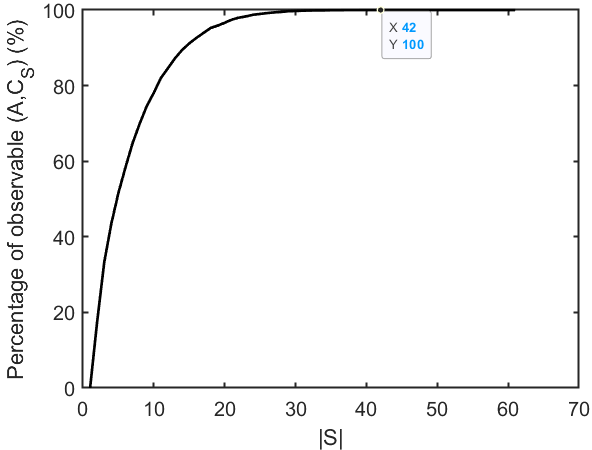
\includegraphics[width=0.82\columnwidth]{new_sim_image/observability.png}
    \caption{Empirical frequency of observability as a function of the number of retained measurements (50,000 random subsets per cardinality).}
    \label{fig:observability}
\end{figure}

All sampled subsets containing at least 42 measurements were observable. This observation motivates the empirical design value $k_0=42$; it does not constitute an exhaustive verification of A2. With $m=61$, the corresponding empirical sparsity guideline is $k\le19$. Experiments with more than 19 attacked channels lie outside the sampled operating regime.

\subsection{Localization performance}
Two four-layer MLPs were evaluated. MLP1 was trained using random additive attacks; MLP2 used the same data augmented with attacks produced by the earlier residual-based physics-guided generator. Thus, this experiment evaluates the general benefit of physics-guided data augmentation, rather than the revised generator in Section~\ref{sec:attack_generation}. Both networks contain three hidden layers with 512, 1024, and 512 ReLU units, followed by an $m$-dimensional sigmoid layer. The comparison uses a common test set of 50,000 FDIAs.

\begin{figure}[!ht]
    \centering
    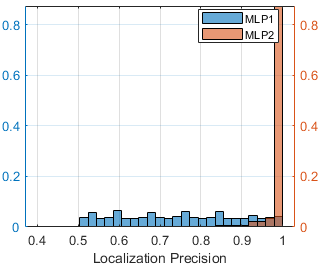
\includegraphics[width=0.78\columnwidth]{new_sim_image/MLP_compare.png}
    \caption{Distribution of channel-localization precision on a common test set. MLP1 is trained using random attacks; MLP2 is trained using random and physics-guided attacks.}
    \label{fig:MLP_compare}
\end{figure}

The mean localization precision increased from $74.37\%$ for MLP1 to $98.69\%$ for MLP2 on the reported test distribution. Together with the empirical value $k_0=42$, calibrated classifier scores would determine the admissible reliability $\eta_{\rm obs}$ through \eqref{equ:eta_observability}. The archived experiment did not record the conditional calibration data or subset Riccati covariances required to evaluate this relation; consequently, no clean-set probability or KF covariance certificate is claimed for these results.
